\section*{Evidenziatore in LaTeX}

\subsection*{1. Evidenziatore giallo (default)}
Questo è un testo \hl{evidenziato in giallo}.

\subsection*{2. Cambiare colore dell'evidenziatore}

\textbf{Azzurro:}\\
{\sethlcolor{cyan!30}\hl{Testo evidenziato in azzurro}}

\vspace{5pt}
\textbf{Rosa:}\\
{\sethlcolor{pink}\hl{Testo evidenziato in rosa}}

\vspace{5pt}
\textbf{Verde chiaro:}\\
{\sethlcolor{green!30}\hl{Testo evidenziato in verde chiaro}}

\vspace{5pt}
\textbf{Arancione:}\\
{\sethlcolor{orange!40}\hl{Testo evidenziato in arancione}}

\subsection*{3. Evidenziare in modalità matematica}

\textbf{Formula evidenziata:}\\
\colorbox{yellow}{$E = mc^2$}

\vspace{5pt}
\colorbox{cyan!30}{$\int_0^1 x^2\,dx$}

\subsection*{4. Legenda colori (modificabili)}

\begin{itemize}
  \item \texttt{yellow} = giallo
  \item \texttt{cyan!30} = azzurro
  \item \texttt{pink} = rosa
  \item \texttt{green!30} = verde chiaro
  \item \texttt{orange!40} = arancione
  \item ... puoi usare anche \texttt{red}, \texttt{blue!20}, \texttt{purple!40}, ecc.

  
\end{itemize}


\begin{figure}[ht]
    \centering
    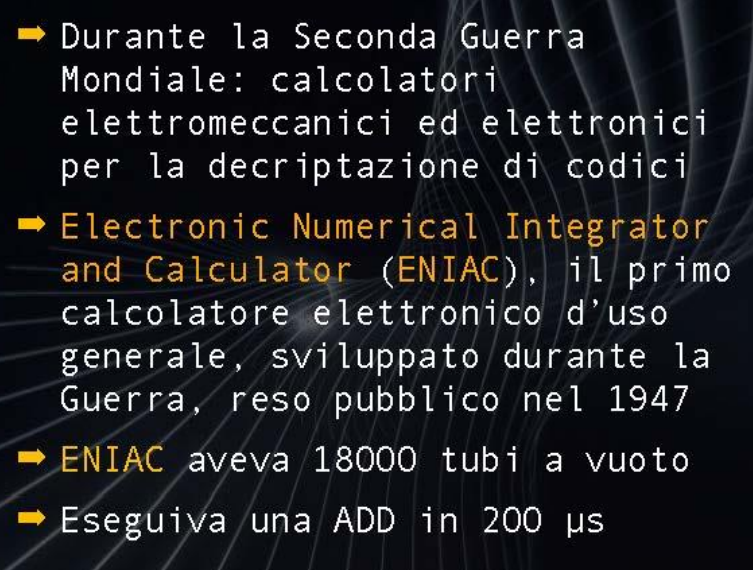
\includegraphics[width=0.9\linewidth]{images/Lez01_fig_01.png}
    \caption{Descrizione URL}
    \label{fig:descrizione_URL}
\end{figure}

\textit{Testo corsivo}